\documentclass{article}

\usepackage[utf8]{inputenc}
\usepackage{ngerman}

\usepackage{graphicx}
\usepackage{subfigure}

\usepackage{lipsum}
\usepackage{pdfpages}

\usepackage{color}
\usepackage{float}

\usepackage{varioref}
	\labelformat{figure}{Abbildung~#1}
	
	

\begin{document}
%opening
\includepdf{TitlePageGDD}
%\newpage
%\tableofcontents
%\newpage

	

\newpage
\section{Genre}

Jump 'n' Run / Roquelike

\vspace{1cm}
\section{Erfolgskriterien}

   \begin{table}[H]
	\centering
	\begin{tabular}{p{4cm}p{7cm}}
		\textbf{Kriterium}  & \textbf{Validierung und Verifikation} \\
		\hline
		\textit{Drei spielbare Level mit unterschiedlicher Optik}          & \textnormal{Eine .exe liefert das Spiel mit 3 oder mehr Leveln, die nacheinander durchgespielt werden können und sich nicht gleich anfühlen}            \\
		\hline
		\textit{Herausfordernd aber nicht zu schwer}       & \textnormal{Playtest mit Freunden und Kursteilnehmern, bei dem es keiner im ersten Anlauf schafft, aber mindestens einer beim 3. Anlauf} \\
		\hline
		\textit{stimmiges Feeling (Grafik, Sound und Gameplay)}        & \textnormal{Durch Interview mit Spieletester/ Befragung nach Vorführung mit kurzer Bewertung} \\
	\end{tabular}	
	\label{tbl:ktierien}
	% Verweis im Text mittels \ref{tbl:beispieltabelle}
	
\end{table}


\vspace{1cm}
\section{Set und Setting}

Wir befinden uns in einer dämonischen Welt in den Gemäuern und Hallen eines unterirdischen Herrschers. Alles ist eher gruselig inszeniert und lebt vom Spiel mit dunklen Klängen und einer tödlichen Umgebung.

\vspace{1cm}
\section{Story}

Der Spieler wurde vom Dämonenlord “Dreg Naffets” gefangen genommen und in einen
Kerker tief im Dämonenreich eingesperrt. Um der bevorstehenden ewigen Folter zu
entkommen, entschließt sich unser Held in einem unbeobachteten Moment den
Zellenwächter zu überwältigen und versucht den Fängen der Dämonen zu entkommen. \newline
Dabei durchquert er die unterschiedlichsten Bereiche der Unterwelt und muss sich mit
verschiedenen Hindernissen und Fallen auseinandersetzen, um seine Flucht zum Erfolg zu führen. \newline
Doch der Dämonenlord verfügt über einen tödliche Macht: der Schleier des Todes - ein Nebel der sich mit hoher Geschwindigkeit ausbreitet und alles Leben vertilgt, dass ihm zu Nahe kommt. \newline
Der Protagonist hat keine Zeit das Verhalten von Fallen zu studieren. Es zählt nur Laufen und Reagieren! Je näher der Held seiner Freiheit kommt, um so schwieriger
werden Fluchtweg und Hindernisse.  \newline
So ist der Held neben seiner Hetzjagd auch noch
gezwungen, Schlüssel zu finden, Sprengstoff für verschlossene Gänge zu sammeln und verlorene Seelen einzufangen, um die große Pforte des Dämonenreiches öffnen zu können. \newline
Doch wenn das alles nicht schon schwer genug wäre, schickt der dunkle Herrscher seine
Schergen los,

\subsection{Spielziel}

Entkomme aus der Dämonenwelt so schnell wie möglich!
Verbessere deine Zeit und deinen Score!

\vspace{1cm}
\section{Gameplay}

\subsection{Kernmechaniken}

Rennen: Der Spieler läuft automatisch und steuert lediglich die Seitwärtsbewegung und
bestimmt so, auf welcher Lane die Spielfigur läuft \newline
Springen: Um Hindernissen, wie z.B. Löchern auszuweichen, kann der Spieler einen
einfachen Sprung ausführen \newline
Rutschen: Dies ist eine Fähigkeit mit der der Spieler unter Barrikaden und Hindernissen hindurch schlittern kann.


\subsection{Meta-Game}

Die Spielwelt besteht aus Gängen, die in vier Lanes aufgeteilt sind. Horizontal wird das
Spiel in ein virtuelles Grid eingeteilt, im Folgenden “Züge” genannt. Pro Zug und Lane kann
immer nur ein Hindernis platziert werden. Eine Lane pro Zug wird als Feld bezeichnet. Es
muss nach jedem Zug immer mindestens ein Feld frei sein, sodass dieses Feld innerhalb eines Zuges (einfacher Lane-Wechsel) erreichbar ist. \newline
Der Spielercharakter läuft automatisch. Je Tastendruck (links/rechts) wird immer nur eine
Lane gewechselt.
Springen/Rutschen überbrückt immer ein Feld, sodass ein passendes Hindernis überwunden
werden kann. \newline
Der Todesschleier breitet sich gleichmäßig aus und ist im normalfall minimal langsamer als
die Standardgeschwindigkeit des Spielers. Der Todesschleier zerstört sämtliche
GameObjects, die er berührt - Also neben der Spielerfigur auch Map, Fallen, Gegner und Co. \newline
Es gibt zwei Arten von Fallen: Debuff und Instant-Death. Debuffs werden die
Laufgeschwindigkeit des Protagonisten zeitweise verringern, so dass der Todesschleier näher
kommt. Instant-Death führt zum sofortigen Tod und damit zum GameOver-State mit der
Eigenschaft “lost”. \newline
Gegner, die der Spieler berührt führen standardmäßig zum sofortigen Tod, können aber mit
einer temporären Waffe (begrenzte Haltbarkeit) bekämpft werden. Dies geschieht
automatisch, sobald der Spieler im Besitz einer Waffe ist und einen Gegner berührt. Dabei
wird der Waffe auch ein Teil ihrer Haltbarkeit abgezogen. \newline
Es gibt teilweise Ressourcen, die während des Laufens aufgesammelt werden müssen, um
ins nächste Level zu gelangen. Es gibt mehr Ressourcen als benötigt werden, um
kleine Fehler zu verzeihen. \newline
Am Ende jeden Levels wird die benötigte Zeit in einen Score umgewandelt und falls alle
notwendigen Bedingungen erfüllt sind (ggf. Collectables), kann das nächste Level gestartet werden. Ein Score aus Collectables wird ermittelt. Die Zeit des Spielers wird bewertet und gegebenenfalls erhält er einen Zeitbonus auf seinen Score.
Andernfalls kann der Spieler das Level wiederholen. \newline
Hat der Spieler alle Level geschafft, erscheint der GameOver-State mit der Eigenschaft “won” und einer abschließenden Statsitik mit Score und Anzahl Toden.

\subsection{Hardmode}

Als eventuelle zusätzliche Schwierigkeit ist ein Hardmode geplant, in dem die Laufgeschwindigkeit des Spielers stark erhöht ist und auch das Einholen des tödlichen Schleiers wesentlich schneller erfolgt. Selbst kleine Fehler werden hier kaum verziehen.

\vspace{1cm}
\section{Struktur des Spiels}

Wie in \ref{fig:gamestates} zu erkennen, gibt es ein Interface (IGameStates) von dem alle Zustände des Spiels erben, sodass sie alle mit den gleichen Funktionen des Game-Loops ausgestattet sind. \newline
Als Einsteigspunkt dient bei uns das Hauptmenü. VOn hieraus kann der Spieler verschiedene Untermenüs erreichen, z.B. Einstellungen (Schwierigkeit, Lautstärke), Statsitik oder Credits.
Natürlich Gibts im Hauptmenü auch die Möglichkeit das Spiel zu beenden und die wichtigste Funktion - Starten des Hauptspiels.
Nach jedem Level wird dem Spieler ein Fortschrittsfenster angezeigt, in dem ihm mitgeteilt wird, ob er das Level wiederholen muss oder weiter spielen kann.
im positivem Falle bestätigt der Gegner den Eintritt ins nächste Level. Bis er schließlich das letzte Level erfolgreich absolviert hat und zum GameOver-Screen kommt mit der Gewinn-Nachricht. Der GameOver-Screen wird aber auch auch bei jeder Niederlage (z.B. Tod des Spielers) angezeigt, allerdings dann natürlich mit der Nachricht des Versagens.

\begin{figure}[H]
	\centering
	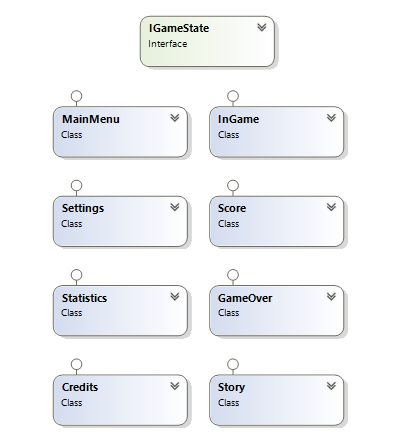
\includegraphics[width=1\textwidth]{gamestates}
	\caption{GameStates -  Veil of Death
		\label{fig:gamestates}}
\end{figure}

\vspace{1cm}
\section{Feedback}

\subsection{Visuell}
Eine GUI unterstützt die Visualisierung des Levelfortschrittes durch Anzeige der Entfernung
zum Ziel als Strecke mit Icon als Spielerrepräsentation und ggf. eine Fortschrittsanzeige (in \%) für notwendige Bedingungen zum Levelabschluss (z.B.: “Finde 10 Coins um den Wächter an der Tür zu bestechen”). \newline
Die Fähigkeiten “Springen” und “Rutschen” erhalten eigene Animationen. \newline
Wird der Spieler verlangsamt oder bekommt einen Power-Up, wird dies durch Spezialeffekte verdeutlicht. \newline
Je Näher der Schleier dem Spieler kommt, umso weniger ist vom Bildschirm zu sehen. Unterstützt wird dies durch Spezialeffekte

\subsection{Akustisch}
Der Spieler erhält bei jeder Auswahl oder Bestätigung eines Menüpunktes o.ä. UI-Element ein akustisches Signal, damit er weiß, dass seine Aktion/Eingabe erfolgreich war. \newline
Die verschiedene Bewegungen werden mit unterschiedlichen Sounds unterlegt, so hört man z.B. ein Wenn der Spieler abspringt und wieder aufkommt jeweils einen eindeutiges Geräusch. \newline
auch die Verfolgung des Schleiers bekommt akustische Signale, so ertönt ein wiedererkennbares Signal, sobald der Schleier in die nächste Phase (Abhängig vom Abstand zum Spieler) übergeht. Zusätzlich dazu erhöht sich die Frequenz des Herzschlags des Spielers, je näher der Schleier kommt.

\subsection{Haptisch}

Beim Spielen mit einem Controller, wird als zusätzliches Feedback die Vibrationsfunktion
des Controllers angesteuert. \newline
Bei Verlangsamung oder PowerUp wird eine mittelkurze Impuls-Vibration getriggert. \newline
Beim Tod des Spielers (egal wodurch) signalisiert ein langes durchgezogenes Vibrieren die
Niederlage. \newline
Ist ein Level erfolgreich absolviert, erhält der Spieler Rückmeldung durch mehrere kurze
aufeinander folgende Vibrationen.

\vspace{1cm}
\section{Ausführliche Beschreibung}

\subsection{Fallenarten und Hindernisse}
Eines der ersten Hindernisse, die der Held kennenlernt sind die Spikes. Das sind Pfähle, die
im Boden versenkt sind und ggf. spontan nach oben stechen. \newline
Eine besondere Art der Falle ist die Kategorie Verlangsamen. Hier sind verschiedenste
Ausprägungen vorstellbar, z.B. Pech, Spinnenweben, Betäuben. Es dient dazu den Vorsprung
des Spielers zum Todesschleier zu verringern. \newline
Als weitere tötende Falle dienen sich drehende und bewegende Säulen, die mit Spitzen bestückt sind. \newline
Als gemeines Gimmick kommt das “böse TNT” hinzu. Im Minen Level
muss der Spieler Dynamit sammeln, um versperrte Gänge frei zu sprengen. Jedoch sehen sich
“gutes TNT” und “böses TNT” verdammt ähnlich. So wird der Spieler in den Tod gerissen,
sammelt er in der Hektik der Flucht den falschen Sprengstoff auf.

\subsection{Buffs und Boni}
Es gibt versteckte Special Items, die eingesammelt werden können und innerhalb 30 sek.
benutzt werden müssen, bevor sie verschwinden. Es rennt sich halt schwer, wenn man die
ganze Zeit Schild oder Schwert mit sich rumschleppt. die Item besitzen eine Haltbarkeit und
nutzen sich bei Gebrauch ab. je nach Seltenheit des Items, hält es 1- 3 Nutzungen, bevor es
zerbricht und verschwindet. \newline
Je nachdem wie schnell der Spieler ein Level absolviert, kann er einen Zeitbonus in drei Abstufungen erhalten.

\subsection{Belohnung und Bestrafung}
Unsere Hauptbelohnung ist die Zeit, je schneller wir ein Level abschließen, umso besser wird
unsere Endwertung. Als weiteren Anreiz, von der Ideallinie
abzuweichen sind versteckte Truhen und Geheimnisse in den Gängen versteckt, die auf den
Score drauf gerechnet werden. \newline
Die offensichtlichste und strengste Bestrafung ist der Tod durch verschiedenste Fallen und
Gegner. Hier verliert der Spieler alle im Level gesammelte Coins und jeglichen anderen Fortschritt. Das Level muss wieder von vorn gestartet werden. \newline
eine weitere Bestrafung ist das Verlangsamen durch Fallen o.ä.. Das wirkt zunächst nicht weiter schlimm. Je öfter wir allerdings verlangsamt werden, um so mehr holt der
Todesschleier den Spieler ein und tötet ihn bei Berührung.

\subsection{Score}
Zunächst erfolgt die Wertung der Zeit in mehreren Abstufungen:
Bestzeit - 1000 Punkte
Silber-Belohnung - 500 Punkte
Bronze-Belohnung - 250 Punkte
Zusätzlich können Schätze gefunden werden, die zufällig jeweils zwischen 50 und
250 Gold (= 50-250 Punkte) enthalten können.
weiter Boni werden für das erfolgreiche Einsetzen der Special-Items vergeben. so
zum Beispiel erhält der Spieler für das Töten eines Gegners mit dem Schwert 100
Punkte.

\subsection{Charaktere}
Unser menschlicher Protagonist heißt Nero und zeichnet sich aus durch starkes
Selbstbewusstsein und seinen erbarmungslosen Überlebenswillen. \newline
Dreg Naffets steht als Antagonist und Dämonenlord auf der anderen Seite
unsers Spiels.
Er hat ungeahnte dunkle Kräfte und befehligt eine riesige Armee von dämonischen Gestalten
und verzauberten Kreaturen. In seinem Schloss verbirgt sich jede Menge Reichtum, allerdings
sind die Zugänge dazu mit Hindernissen und tödlichen Fallen gespickt.
Als Pseudo-Charakter sei hier noch der Schwarze Nebel, der “Todesschleier”, als gefährlichste
Macht Dregs erwähnt. Einmal entfesselt, breitet sich die Schattenwolke gleichmäßig aus und
schleicht durch die Welt um alles, was sie berührt leise zu töten. Diese Wolke ist die
antreibende Kraft unserer Flucht, denn lässt sich unser Held zu viel Zeit, holt der Nebel uns
ein und wird uns vertilgen.

\vspace{1cm}
\subsection{Orte}
\subsubsection{“Kerker des Schreckens”}
Hier startet das Spiel. Im Gang entlang findet man immer wieder weitere Gefangenenzellen. \newline
\subsubsection{“Festung der Hoffnungslosigkeit”}
Dies ist der Palast des Königs. Nachdem unser Protagonist aus dem Kerker entkommen ist,
führt seine Flucht durch die verschiedenen Ebenen des Palastes, vorbei an Wachen und
lebensgefährlichen Fallen. Wer trotz der Panik aufmerksam ist, wird im Palast viele versteckte
kostbare Gegenstände oder vielleicht auch Power-Ups finden. \newline
\subsubsection{“Minen der Einsamkeit”}
Aus dem Palast entkommen, führt der Weg durch die Arbeitslager und Minen. viele morsche
bausubstanz birgt hier ein hohes Risiko durch herunterfallende Decken und Sprengstoff.
Dieser kann zum einen eingesammelt werden, um versperrte Bereiche zu sprengen. Allerdings
sind unter den TNT-Stangen auch oft Blindgänger, die das Leben und damit die Flucht unseres
Helden beenden. \newline
\subsubsection{“Wald der Düsternis”}
Im vorletzten Abschnitt unserer Flucht führt es uns durch einen dichten Wald. Überall lauern
gefahren, wie z.B. verdorbene Kreaturen des Waldes. Zusätzlich befinden sich überall
Spinnennester, die zum einen dir deine Loot klauen und zum anderen Spinnenweben, die dich
verlangsamen, sodass der dunkle Schleier näher rückt. \newline
\subsubsection{“Ebene der Grausamkeit”}
Um zum Tor der Dämonenwelt zu gelangen, um endgültig auszubrechen, müssen wir durch
eine virtuelle Ebene. Diese ist als innere oder geistige Dimension zu verstehen und spieglet quasi den "Endkampf" mit den Auswirkungen des tödlichen Schleiers dar.
Der Dämonenlord - erzürnt durch die Flucht - lässt all seine dämonischen Mächte auf dich los, um dich mit allen Mitteln aufzuhalten.

\vspace{1cm}	
\section{Unique Selling Points}
\begin{itemize}
	\item{Runner im dämonsichen Setting mit stimmiger grafischer und akustischer Untermalung}
	\item{Runner mit echter Story}
	\item{Durch ausreichend visuelles und akustisches Feedback entsteht ein immersives Spiel}
\end{itemize}

	
\end{document}



